\hypertarget{realCompare_8h}{
\section{real\-Compare.h File Reference}
\label{realCompare_8h}\index{realCompare.h@{realCompare.h}}
}
{\tt \#include $<$stdio.h$>$}\par
{\tt \#include $<$stdlib.h$>$}\par
{\tt \#include $<$string.h$>$}\par
{\tt \#include $<$errno.h$>$}\par
{\tt \#include $<$gsl/gsl\_\-matrix.h$>$}\par
{\tt \#include \char`\"{}real\-Io.h\char`\"{}}\par
{\tt \#include \char`\"{}bit\-Set.h\char`\"{}}\par
{\tt \#include \char`\"{}prot\-Align.h\char`\"{}}\par


Include dependency graph for real\-Compare.h:\begin{figure}[H]
\begin{center}
\leavevmode
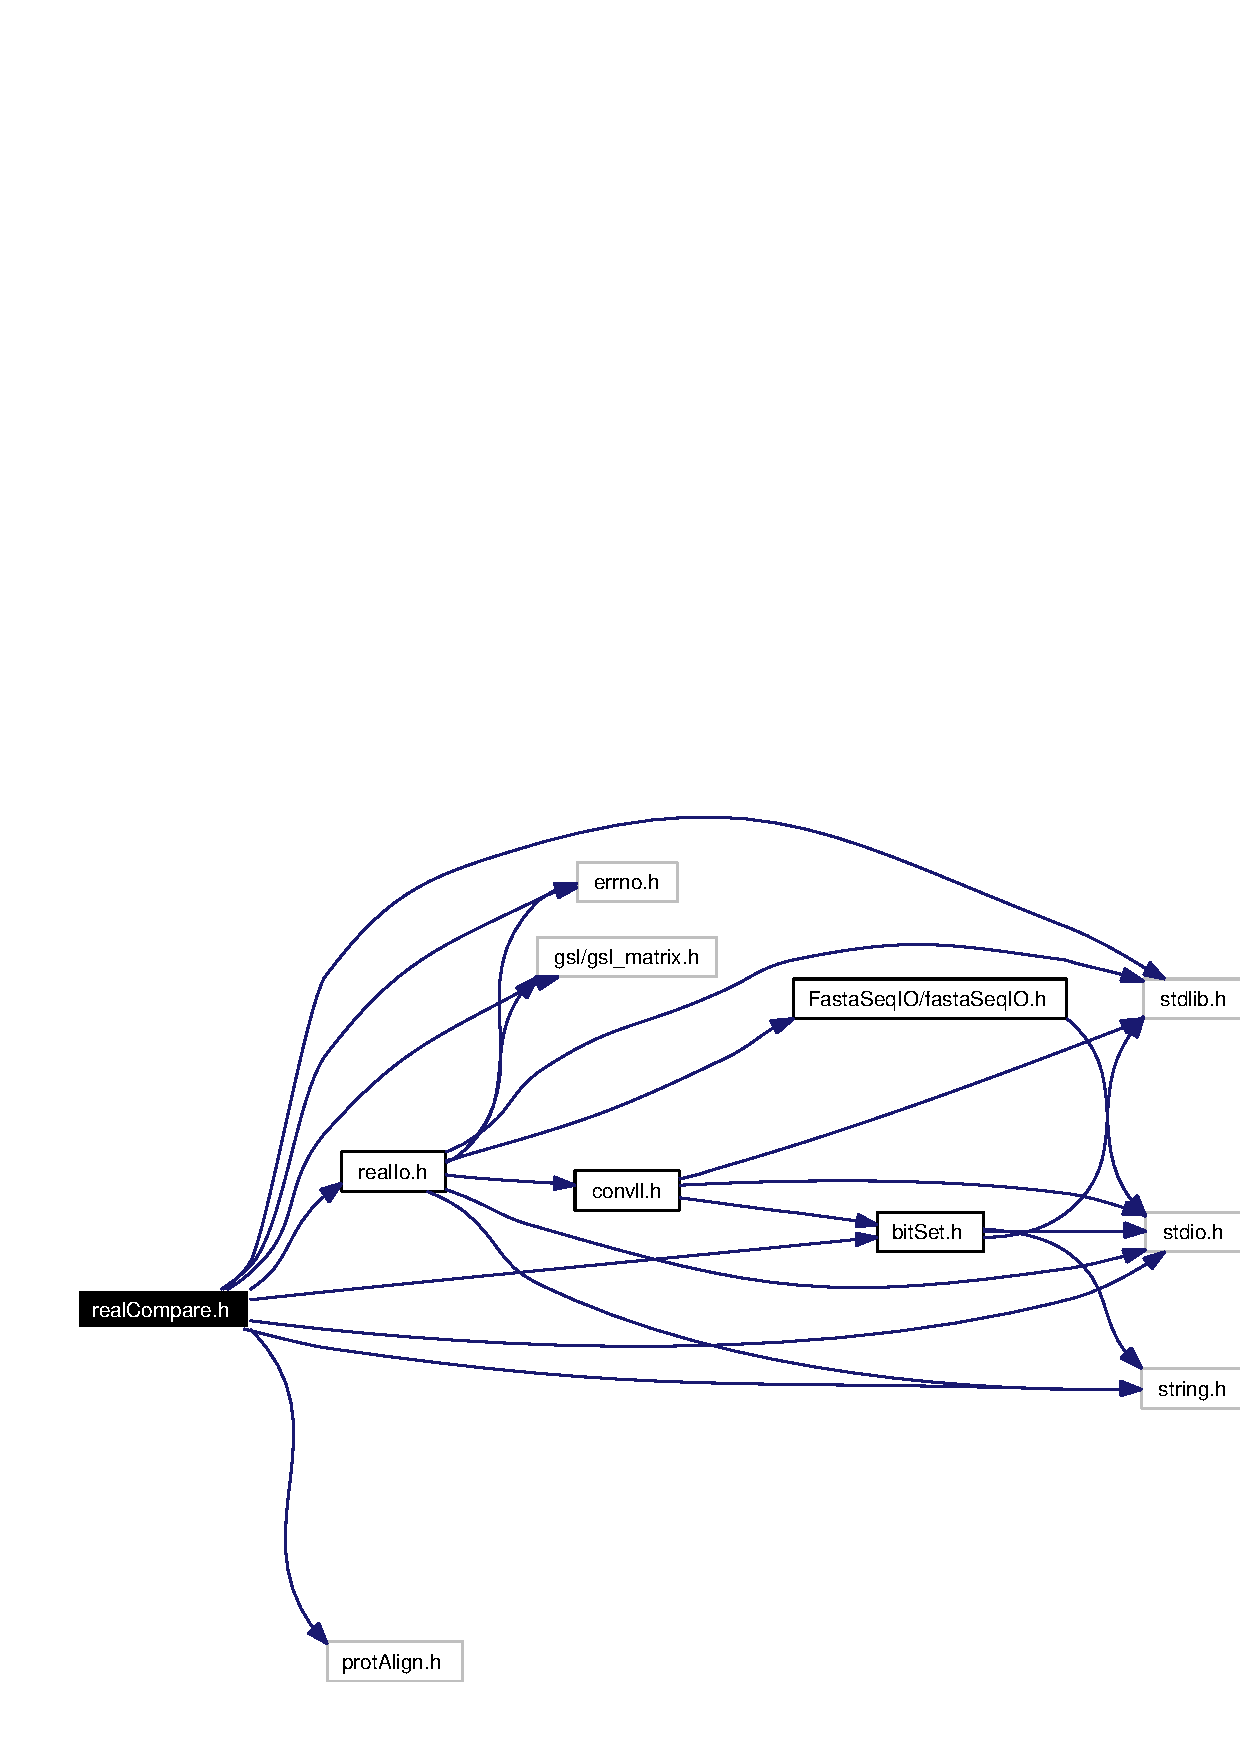
\includegraphics[width=299pt]{realCompare_8h__incl}
\end{center}
\end{figure}


This graph shows which files directly or indirectly include this file:\begin{figure}[H]
\begin{center}
\leavevmode
\includegraphics[width=119pt]{realCompare_8h__dep__incl}
\end{center}
\end{figure}
\subsection*{Functions}
\begin{CompactItemize}
\item 
double \hyperlink{realCompare_8h_a1}{rmsd\-Compare} (\hyperlink{structrdh__t}{rdh\_\-t} $\ast$data, int win1, int win2, int L, double $\ast$extra\-Params)
\item 
double \hyperlink{realCompare_8h_a2}{general\-Match\-Factor} (\hyperlink{structrdh__t}{rdh\_\-t} $\ast$data, int win1, int win2, int L, double $\ast$extra\-Params)
\item 
double \hyperlink{realCompare_8h_a3}{mass\-Spec\-Compare\-WElut} (\hyperlink{structrdh__t}{rdh\_\-t} $\ast$data, int win1, int win2, int L, double $\ast$extra\-Params)
\item 
\hyperlink{structbitGraph__t}{bit\-Graph\_\-t} $\ast$ \hyperlink{realCompare_8h_a4}{real\-Comparison} (\hyperlink{structrdh__t}{rdh\_\-t} $\ast$data, int l, double g, int comp\-Func, double $\ast$extra\-Params)
\end{CompactItemize}
\subsection*{Variables}
\begin{CompactItemize}
\item 
double($\ast$)(\hyperlink{structrdh__t}{rdh\_\-t} $\ast$, int, int, int, double $\ast$) \hyperlink{realCompare_8h_a0}{get\-Comp\-Func} (int comp\-Func)
\end{CompactItemize}


\subsection*{Detailed Description}
This file contains declarations and definitions used for the comparison of real valued data during the comparison phase of Gemoda. The functions declared here are defined in \hyperlink{realCompare_8c}{real\-Compare.c}.

Definition in file \hyperlink{realCompare_8h-source}{real\-Compare.h}.

\subsection*{Function Documentation}
\hypertarget{realCompare_8h_a2}{
\index{realCompare.h@{real\-Compare.h}!generalMatchFactor@{generalMatchFactor}}
\index{generalMatchFactor@{generalMatchFactor}!realCompare.h@{real\-Compare.h}}
\subsubsection[generalMatchFactor]{\setlength{\rightskip}{0pt plus 5cm}double general\-Match\-Factor (\hyperlink{structrdh__t}{rdh\_\-t} $\ast$ {\em data}, int {\em win1}, int {\em win2}, int {\em L}, double $\ast$ {\em extra\-Params})}}
\label{realCompare_8h_a2}


This function is used to compute a generalized match factor, which is useful for computing the degree of similarity between mass spectrometry spectra.

Definition at line 111 of file real\-Compare.c.

References get\-Rdh\-Dim(), get\-Rdh\-Index\-Seq\-Pos(), and rdh\_\-t::seq.

Referenced by get\-Comp\-Func().



\hypertarget{realCompare_8h_a3}{
\index{realCompare.h@{real\-Compare.h}!massSpecCompareWElut@{massSpecCompareWElut}}
\index{massSpecCompareWElut@{massSpecCompareWElut}!realCompare.h@{real\-Compare.h}}
\subsubsection[massSpecCompareWElut]{\setlength{\rightskip}{0pt plus 5cm}double mass\-Spec\-Compare\-WElut (\hyperlink{structrdh__t}{rdh\_\-t} $\ast$ {\em data}, int {\em win1}, int {\em win2}, int {\em L}, double $\ast$ {\em extra\-Params})}}
\label{realCompare_8h_a3}


This function is used to compute the match factor between to mass spectrometry spectra in a similar manner to the previous function; however, this function imposes a penalty for spectra that are separated by large distances in elution time. This function is commonly used by Spec\-Connect.

Definition at line 174 of file real\-Compare.c.

References get\-Rdh\-Dim(), get\-Rdh\-Index\-Seq\-Pos(), and rdh\_\-t::seq.

Referenced by get\-Comp\-Func().



\hypertarget{realCompare_8h_a4}{
\index{realCompare.h@{real\-Compare.h}!realComparison@{realComparison}}
\index{realComparison@{realComparison}!realCompare.h@{real\-Compare.h}}
\subsubsection[realComparison]{\setlength{\rightskip}{0pt plus 5cm}\hyperlink{structbitGraph__t}{bit\-Graph\_\-t}$\ast$ real\-Comparison (\hyperlink{structrdh__t}{rdh\_\-t} $\ast$ {\em data}, int {\em l}, double {\em g}, int {\em comp\-Func}, double $\ast$ {\em extra\-Params})}}
\label{realCompare_8h_a4}




Definition at line 272 of file real\-Compare.c.

References bit\-Graph\-Set\-True\-Sym(), get\-Comp\-Func, get\-Rdh\-Index\-Seq\-Pos(), rdh\_\-t::index\-Size, init\-Rdh\-Index(), new\-Bit\-Graph(), and rmsd\-Compare().

Referenced by main().



\hypertarget{realCompare_8h_a1}{
\index{realCompare.h@{real\-Compare.h}!rmsdCompare@{rmsdCompare}}
\index{rmsdCompare@{rmsdCompare}!realCompare.h@{real\-Compare.h}}
\subsubsection[rmsdCompare]{\setlength{\rightskip}{0pt plus 5cm}double rmsd\-Compare (\hyperlink{structrdh__t}{rdh\_\-t} $\ast$ {\em data}, int {\em win1}, int {\em win2}, int {\em L}, double $\ast$ {\em extra\-Params})}}
\label{realCompare_8h_a1}


Calculate the rmsd between two windows, with optional translation and rotation. The input to this function is a real data handler object, two integers that point to the windows within the real data that are to be compared, an integer that specifies the length of the windows, and a pointer to a double precision floating point that can be used to store other parameters as needed. This last parameter is most useful for implementing other comparison functions, without having to make, too many changes to other parts of the code.

This function operates in three stages. First, we compute the centroid of each window and move the second window such that its centroid overlaps with that of the first window. Second, we use rigid body rotation to find the rotational matrix that minimizes the root mean squared deviation between the two windows. Finally, this function returns that minimized RMSD.

Definition at line 31 of file real\-Compare.c.

References get\-Rdh\-Dim(), get\-Rdh\-Index\-Seq\-Pos(), and rdh\_\-t::seq.

Referenced by get\-Comp\-Func(), and real\-Comparison().





\subsection*{Variable Documentation}
\hypertarget{realCompare_8h_a0}{
\index{realCompare.h@{real\-Compare.h}!getCompFunc@{getCompFunc}}
\index{getCompFunc@{getCompFunc}!realCompare.h@{real\-Compare.h}}
\subsubsection[getCompFunc]{\setlength{\rightskip}{0pt plus 5cm}double($\ast$)(\hyperlink{structrdh__t}{rdh\_\-t}$\ast$, int, int, int, double$\ast$) get\-Comp\-Func(int comp\-Func)}}
\label{realCompare_8h_a0}




Definition at line 36 of file real\-Compare.h.

Referenced by find\-Clique\-Centroid(), output\-Real\-Pats\-WCentroid(), and real\-Comparison().
